\chapter{Introducci\'on}

\label{Chapter1}

La intro la podes pensar en 3 subsecciones: descripción de elecciones y contabilización de las actas hoy, la
oportunidad que se presenta con la digitalización (y los desafíos que aparecen) y luego los objetivos. Tiene que quedar
claro que problema ves y qué propones hacer a grandes rasgos. También es importante que estos objetivos se vean
reflejados en los resultados y conclusiones (es decir, prometer algo que después cumplis al final del doc)

\section{Contexto}

En Argentina se celebran elecciones cada 2 a\~{n}os a excepci\'on de las presidenciales que se realizan cada 4
a\~{n}os. Existen, principalmente, tres tipos de elecciones:

\begin{itemize}
    \item Elecciones nacionales, para elegir a las autoridades federales del país: el Poder Ejecutivo, constituido por el
          Presidente y el vicepresidente y el Congreso Nacional, formado por Senadores y Diputados.
    \item Elecciones provinciales y de la Ciudad de Buenos Aires o locales, para elegir a las autoridades de cada provincia: los
          poderes ejecutivos de las provincias y sus legislaturas.
    \item Elecciones municipales, regidas por las leyes y procedimientos de cada provincia.
\end{itemize}

Si bien emitir el sufragio es diferente en cada una de ellas, generalmente consta de ingresar a un cuarto oscuro,
elegir el candidato que se desea y depositar el voto en una urna. Al finalizar la jornada, las autoridades de mesas
recuentan los votos y llenan una planilla a mano alzada donde se resume la cantidad de votos obtenidos por cada
candidato o partido pol\'itico. Dicha planilla es escaneada y enviada a traves de un telegrama del correo argentino al
centro de c\'omputo para su procesamiento. Una vez all\'i, se contabilizan en un sistema inform\'atico a partir de un
grupo de personas. Este proceso cuenta con una etapa de de digitalizaci\'on y otra de validaci\'on (TODO: esto lo vi en
el diagrama de las elecciones de cordoba. no encontre nada oficial al respecto.).

\begin{figure}[H]
    \centering
    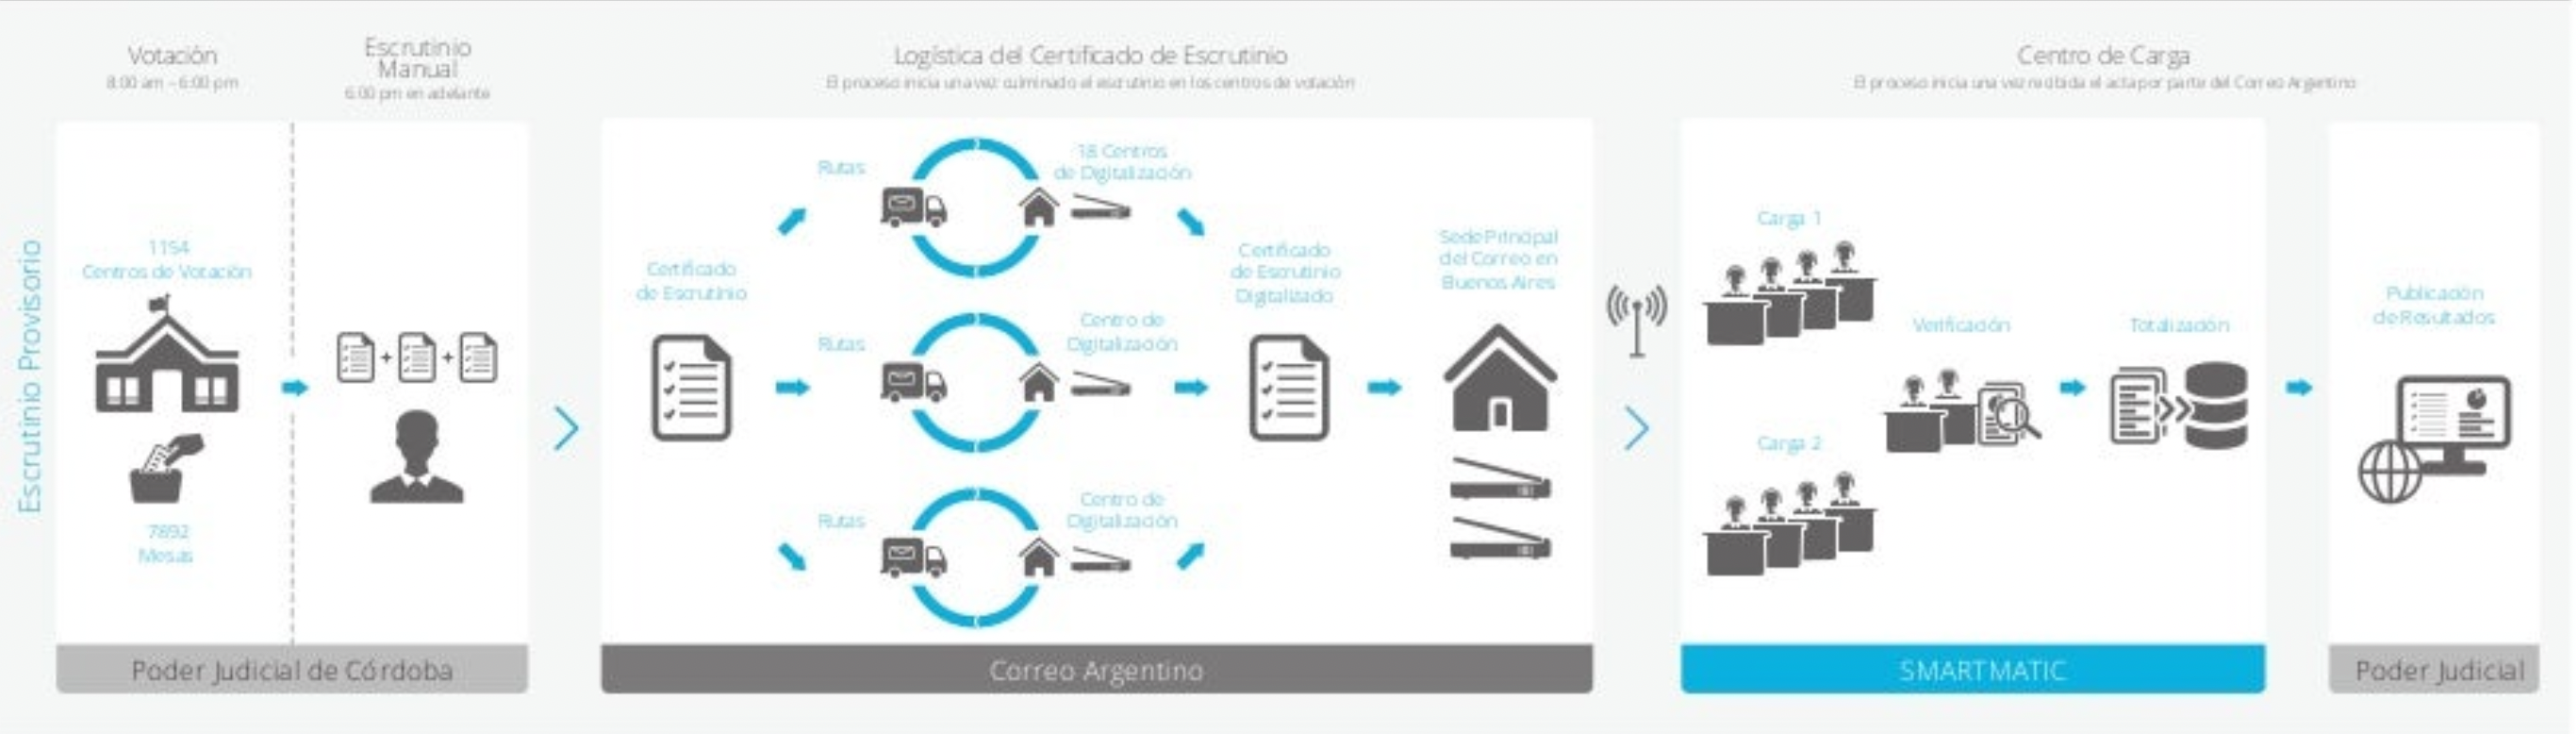
\includegraphics[width=1\textwidth]{chapter1/proceso-elecciones.png}
    \caption{Proceso eleccionario. TODO: cambiar para que se pueda leer o eliminar directament?}
    \label{fig:proceso-elecciones}
\end{figure}

Para que el proceso sea lo mas r\'apido y eficaz posible, se requiere a una gran cantidad personas destinadas al centro
de c\'omputo. Tal soluci\'on hace que el proceso sea altamente ineficiente en cuanto a tiempos y costos se refiere. En
las elecciones legislativas del 2021 se gastaron unos \$17.000 millones de pesos de los cuales \$4.000 millones de
pesos fueron destinados a sueldos para el personal\footnote{Fuente:
    \href{https://www.cronista.com/economia-politica/Elecciones-legislativas-2021-cuanto-mas-se-gastara-por-el-coronavirus-segun-el-Presupuesto-20201004-0006.html}{El
        cronista}}.

\section{Motivaci\'on}

Digitalizar los telegramas de manera autom\'atica supondr\'a un ahorro considerable en el presupuesto de las
elecciones, agilizar\'a la obtenci\'on de los resultados y aportar\'a transparencia al proceso en general. Es posible
entrenar un modelo de clasificaci\'on de d\'igitos a un costo extremadamente menor al actual y utilizarlo al momento de
la contabilizaci\'on de los votos.

Contar con una digitalizaci\'on autom\'atica permitir\'a bajar los costos debido a que se necesitar\'a un grupo menor
de personas en el centro de c\'omputo. Adem\'as, el trabajo a realizar ser\'a mas simple ya que s\'olo constar\'a del
proceso de validaci\'on.

La clasificaci\'on de n\'umeros es un problema que, si bien parece resuelto con \cite{lecun1998gradient} y la
creaci\'on del dataset MNIST, no debe ser tomada a la ligera. No existe una \'unica forma de escribir y a\~{n}o a
a\~{n}o cambian las personas que son los jefes de mesa encargados de completar los telegramas. Las caracter\'isticas de
los n\'umeros escritos a mano difiere entre cada elecci\'on. Cuando la distribuci\'on de los datos de entrenamiento
difiere a la de los datos de aplicaci\'on, se est\'a ante un {\it corrimiento de dominio} ({\it domain shift} o {\it
        data drift} en ingl\'es). Esto implica que un modelo que se entrene en alg\'un dataset est\'atico como el MNIST que fue
creado en el \citeyear{lecun1998gradient}, har\'a malas clasficaciones los d\'igitos de las elecciones.

Cuando los dominios de entrenamiento (origen) y aplicaci\'on (destino) son distintos, se debe a que hay un {\it sesgo}
en los datos. Las t\'ecnicas de entrenamiento cl\'asicas suponen que, si bien existe el sesgo existe, \'este ser\'a el
mismo entre origen y destino. Cuando el supuesto no se cumple, se debe recurrir a t\'ecnicas de entrenamiento m\'as
complejas donde se intenta que el modelo aprenda a adaptar un dominio a otro. Hoy en d\'ia no hay trabajos relacionados
a la digitalizaci\'on de telegramas en Argentina que compare c\'ual es la mejor t\'ecnica de adaptaci\'on de dominio.

\section{Objetivos}

La presente tesis enfocar\'a en el desarrollo de un modelo que permita digitalizar los telegramas de las elecciones en
Argentina utilizando las legislativas de la provincia de Santa Fe del a\~{n}o 2021 como comparativa. Los telegramas son
p\'ublicos y se encuentran subidos en la \href{https://op.elecciones.gob.ar/telegramas/generales2021/}{p\'agina oficial
    del estado argentino}. En el anexo \ref{anexo:telegramas} se adjunta un ejemplo de uno de ellos.

Para poder llevarlo a cabo, se procede a:
\begin{itemize}
    \item Extraer los n\'umeros escritos a mano en los telegramas.
    \item Evaluar t\'ecnicas de adaptaci\'on de dominio para entrenar modelos destinados a la clasificaci\'on de n\'umeros de los
          telegramas.
    \item Analizar los espacios latentes de los modelos con el fin de obtener {\it insights} respecto a la capacidad de
          generalizaci\'on de los modelos.
\end{itemize}